\section{Introduction}
\subsection{Background}
People have been playing mathematical games
since as early as 2000 B.C.
\cite{cornelius1986historical}.
All along,
players have attempted to devise optimal
strategies, simulate future moves, or identify
flaws in logic that can be exploited.
Mathematics can serve as a particularly powerful tool for
such analysis.
Abbott and Richey used Markov Chains
to find the long term 
distribution of turns players spend in different
properties in the board game
\textit{Monopoly} \cite{abbott1997take, magie1935}.
(They also found that the optimal strategy is to avoid making
moves altogether and instead maximize time spent in jail.)
Lyford et al. investigated the probability and expected value 
in the board game \textit{Camel Up}
\cite{bogen2014, lyford2019using}.
Witter and Lyford generated an optimal winning strategy for the 
board game \textit{Codenames} using matrix rotations
and a combinatorial argument \cite{chvatil2015}.
% TO DO: CITE CODENAMES PAPER IF ACCEPTED

Another example of a game with mathematical underpinnings is
the board game \textit{Ticket to Ride} \cite{moon2004ticket}. 
Players race to connect 
cities and build railroads on a map of the U.S.
Mathematically, the board
can be thought of as a graph where
cities represent vertices and the
routes between them represent edges.
The educational implications of \textit{Ticket to Ride}
have been extensively studied.
Lim applied the game to teach basic graph theory
\cite{lim2007taking}.
Chang et al. introduced Kruskal's, Prim's, and Dijkstra's
algorithms in the context of \textit{Ticket to Ride}
\cite{chang2008learning}.
Finally, Drake taught beginning programming skills by having
students implement a digital version 
of the game \cite{drake2011teaching}.
In addition, \textit{Ticket to Ride} 
has been studied in the context of
accessible game design and eye-tracking visualization
\cite{eriksson2005enhancing, newn2017evaluating}.

Previous work has also focused on improving player 
strategies in \textit{Ticket to Ride}.
Silva et al. used simulations to compare different
heuristic strategies \cite{de2017playtesting}.
In related papers, the same authors explore the 
game space to find trends in the way \textit{Ticket to Ride}
is played and experiment with new maps and decks 
\cite{de2017evaluator, de2018evolving}.

We extend the mathematical interpretations of
\textit{Ticket to Ride} to devise better player strategies
and a better scoring scheme.

To investigate a better way to assign points for building routes,
we use a clever application of indicator random variables.
Our approach yields the expected time until certain moves
can be made in the board game.
We then argue that this expected time should be proportional
to the reward for these moves.

To investigate the difficulty of connecting pairs of cities,
we use effective resistance and a statistical model.
In graph theory, effective resistance is a measure of the 
difficulty an electrical current undergoes to travel
between one node and another.
We implement two existing algorithms to calculate
the effective resistances between nodes
\cite{ellens2011effective, wu2004theory}
and apply them to the \textit{Ticket to Ride} board.
By comparing the effective resistance, the reward
of collecting a pair of cities, and the most successful
pairs of cities in simulated games, we suggest
strategies for players to pick the best cities.

The overarching question of this work is as follows:
What mathematical structure in \textit{Ticket to Ride}
can be exploited to optimize player strategies?
Our answer builds on existing results and
our own novel applications of mathematical concepts to enhance
player strategies and propose a better scoring scheme.
% discuss "better"

\subsection{\textit{Ticket to Ride} Gameplay}

\textit{Ticket to Ride} is a a board game for two to five
players and the goal for each player is to collect
the most points by the end of the game.
There are three ways players may accumulate points:
First, a player receives points for building routes
(edges between nodes)
on the board in \cref{fig:board}.
The number of points scored is based on the length of the route
according to \cref{table:current_value}.
Second, a player receives points for building
a set of routes that connect two cities specified
on a Destination Ticket.
(A player must possess the corresponding Destination Ticket to earn
points for connecting two cities.)
Finally, a player receives points for building
the longest path of routes at the end of the game.
(A path connects two cities through a set
of routes and may only use a single route exactly once.)

\begin{figure}[h]
\centering
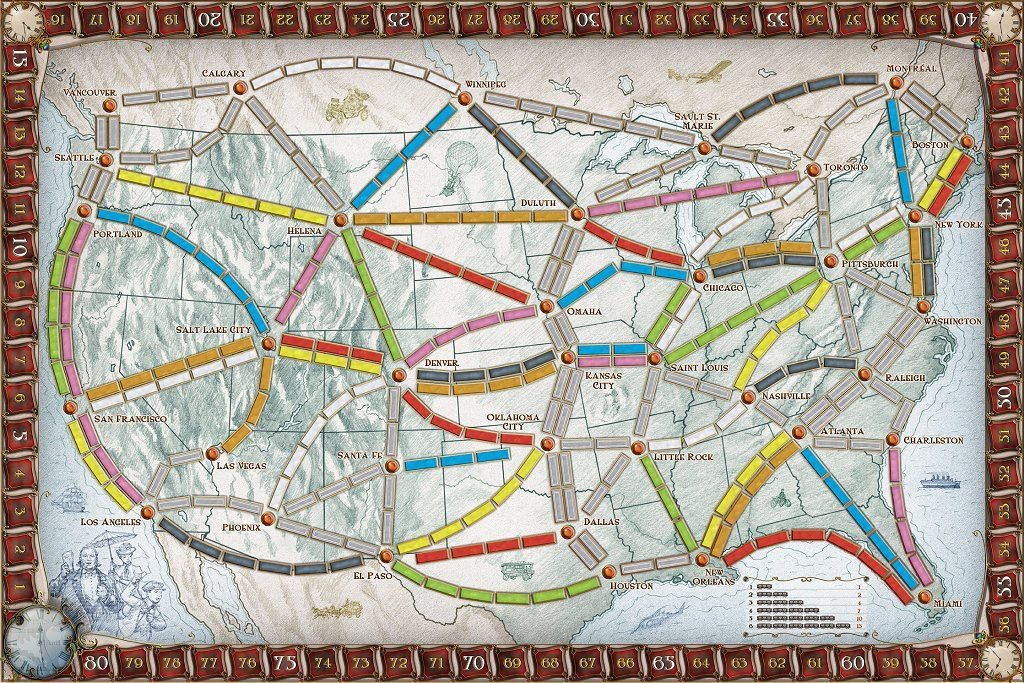
\includegraphics[scale=.4]{figures/board}
\captionof{figure}{The \textit{Ticket to Ride} U.S. board.}
\label{fig:board}
\end{figure}

Each player begins the game with four random Train Car cards.
These cards are used to buy routes.
(There are 110 cards: 12 of eight colors and 14 'wild' cards
that can stand in for any color.)
For example, a player can use four pink Train Car cards to purchase
the route between Charleston and Miami
at the bottom right corner of \cref{fig:board}.
At the beginning of the game 
each player also receives three Destination Ticket cards.
Two cities and a reward are specified on each Destination Ticket.
Players choose either two or three of these cards and
receive points based on whether
or not they complete the Destination Ticket:
if they connect the cities then they add the point reward to their
total score and
if they did not connect the cities by the end of the game they
subtract the points from their total score.

Players take one of three actions each turn.
First, a player may draw two Train Car cards either
from the deck or from the five Train Car cards
kept face up on the table. 
(If a player chooses a wild card from the table
then they are limited to one Train Car card that turn.)
Second, a player may claim a route by trading in
the appropriate number and color of Train Car cards
and placing their own trains on the route.
The gray routes on the map are purchased with
the appropriate number of any one color
and a player may only purchase unclaimed routes.
Finally, a player may draw three Destination Tickets
and return up to two of them.

When one player's stock of 45 trains dips 
below 3 trains after claiming a route,
every player (including that player) gets one final turn.

\subsection{Simulations}
We used Silva et al.'s program to simulate
\textit{Ticket to Ride} games \cite{silva2019}.
We run our simulations on the USA map.
(While there exist other maps, we restrict our analysis
to one map because our results are board specific.)
For simulated four-player games, we include each of 
Silva et al.'s four agent types:
The Destination Hungry Agent chooses 
Destination Tickets at the beginning of the
game--with an emphasis on Destination 
Tickets that are geographically close--
and tries to connect them for the rest of the game.
The Route Focused Agent works toward 
a longer Destination Ticket then claims longer routes.
The One Step Agent operates by choosing 
the most advantageous move at each
step without a long term strategy.
The Long Route Agent claims 
longer routes (defined as four trains or more)
with a preference for routes that help 
connect the player's initial Destination Tickets.
For two-player games, we simulate an equal number 
of all six pairings of the four agents.
Our forked verision of Silva et al.'s
Github repository is publicly available online
\cite{witter2019}.

\subsection{Overview}
\todo{view over}
